\section{Group Controllers}\label{group-controllers}

\subsection{Controls (Air Loop and Zone Equipment)}\label{controls-air-loop-and-zone-equipment}

A controller mimics the function of an actual physical controller in a somewhat rudimentary way. It can sense one node variable, compare it with its setpoint, and determine the desired value for another node variable. It should be noted that a controller cannot span a loop manager boundary (but a Setpoint Manager can). Thus, in an air loop (\hyperref[airloophvac]{AirLoopHVAC}), the sensed node and the controlled device must be in the air loop simulation. This means that a single zone system cannot be modeled with a simple controller sensing zone temperature and controlling coil water flow. Instead this must be modeled as a Setpoint Manager sensing a zone temperature and resetting the supply air temperature setpoint each timestep. This is artificial but should simplify the control modeling task. It should also be noted that there are various types of controllers and that each controller might hook into loops in a slightly different way. As a result, each controller type is described separately below.

\subsection{Controller:WaterCoil}\label{controllerwatercoil}

This controller is really a solution inverter. For a water coil the simulation cannot be inverted where the mass flow rate of the water through the coil can be solved directly given an air temperature. Thus, this controller will numerically step through all of the water flow possibilities by an interval-halving technique until the mass flow rate is determined to meet the specified outlet air temperature within a specified user tolerance.

As the reader probably noted when reading the descriptions of the coil syntax shown earlier in this section, there were no controls attached directly to a particular component. This is because the input can be simplified somewhat by entering node names to be controlled. This avoids having to search through multiple lists of component types for the sake of simply controlling components. The Controller:WaterCoil shown below is a way of controlling variables at one node based on conditions at another node. After the identifying name for the controller, the user must define which control variable the controller is managing. These options include Temperature, Humidity Ratio, TemperatureAndHumidityRatio, or Flow.

The next parameter in the input syntax is the Action of the control, which determines how the controlled variable (e.g., mass flow rate through a water coil) is changed based on the control signal. The following input parameter is the actuator variable, which is currently limited to mass flow through a water coil.

The next two parameters in the input syntax are node names corresponding to the node that is being sensed and the actuated node which controls the water mass flow through the coil. For example, in the case of a cooling coil the control variable might be the outlet air temperature of the coil while the actuated variable might be the water flow rate through the coil. These two parameters are followed by the controller convergence tolerance. Finally, the last two input parameters represent the maximum and minimum values allowed for the actuated variable at the actuated node.

\subsubsection{Inputs}\label{inputs-008}

\paragraph{Field: Name}\label{field-name-007}

This is the unique name of the controller.

\paragraph{Field: Control Variable}\label{field-control-variable}

This was setup to be generic but to date has only been used for temperature control, or temperature and humidity ratio control, of a water coil in the air loop simulation. The keyword Temperature is used for air temperature control and is normally specified for the coils outlet air node. The keyword TemperatureAndHumidityRatio is used for controlling both air temperature and high humidity levels, and is normally specified for a cooling coils outlet air node. The keyword HumidityRatio is used for humidity control and would normally be specified for a dehumidifier outlet node. These two keywords require a \hyperref[zonecontrolhumidistat]{ZoneControl:Humidistat} object and a maximum humidity setpoint manager object (SetPointManager:SingleZone:Humidity:Maximum, SetPointManager:MultiZone:MaximumHumidity:Average or SetPointManager:MultiZone:Humidity:Maximum). If the coil is located in the outdoor air stream, it may also be necessary to use \hyperref[setpointmanageroutdoorairpretreat]{SetpointManager:OutdoorAirPretreat}.

\paragraph{Field: Action}\label{field-action}

The next input refers to the action of the control. This can be best described by an example. In a coil where water mass flow rate is to be controlled, a coil will increase the mass flow rate through the coil when more heating or cooling is requested. In a heating coil, this increases the value of heat transfer from the water to the air stream. As a result, this is considered a Normal action controller. In a cooling coil, an increase in water mass flow rate through the coil decreases the value of heat transfer from the water to the air stream (absolute value increases, but since cooling is traditionally described as a negative number, an increase in absolute value results in a decrease in the actual heat transfer value). Thus, the cooling coil controller has Reverse action since an increase in flow rate results in a decrease in heat transfer.

\paragraph{Field: Actuator Variable}\label{field-actuator-variable}

This was again meant to be more generic but currently has only been used to control the water mass flow rate of a heating or cooling coil. This actuator variable must be set to the keyword Flow to control the water mass flow rate.

\paragraph{Field: Sensor Node Name}\label{field-sensor-node-name}

Name of the node where the temperature, humidity ratio or flow is sensed.

\paragraph{Field: Actuator Node Name}\label{field-actuator-node-name}

Name of the actuated node that controls the water mass flow rate through the coil.

\paragraph{Field: Controller Convergence Tolerance}\label{field-controller-convergence-tolerance}

The coil is controlled by knowing the outlet temperature and/or humidity ratio specified by the setpoint managers, and setting the outlet conditions from the coil to meet these setpoints. The hot and chilled water coils use complex models that cannot be inverted directly. Therefore, to determine the correct mass flow rate for the hot or cold water the models are inverted numerically using an iterative procedure. The iterative solution uses an interval-halving routine and needs a termination criterion that is set with the Controller Convergence Tolerance parameter. The convergence tolerance is the maximum difference between the actual temperature at the setpoint node and the setpoint temperature. This control offset is set to a small temperature difference, such as 0.01 to denote 1/100 degree C. The default is 0.1 degree C.

\paragraph{Field: Maximum Actuated Flow}\label{field-maximum-actuated-flow}

This is the maximum water flow (m\(^{3}\)/sec) through the coil. Set to the maximum design water flow for the coil.

\paragraph{Field: Minimum Actuated Flow}\label{field-minimum-actuated-flow}

Set to the minimum design water flow (m\(^{3}\)/sec) for the water coil, normally a shut off valve that is set to zero.

An example of this object in an IDF, along with appropriate setpoint managers, is shown below:

\begin{lstlisting}

Controller:WaterCoil,
  Central Cooling Coil Controller 1,    !- Name
  TemperatureAndHumidityRatio,          !- Control Variable
  Reverse,                              !- Action
  Flow,                                 !- Actuator Variable
  VAV Sys 1 Outlet Node,                !- Sensor Node Name
  Main Cooling Coil 1 Water Inlet Node, !- Actuator Node Name
  0.002,                                !- Controller Convergence Tolerance {deltaC}
  0.025,                                !- Maximum Actuated Flow {m3/s}
  0.0;                                  !- Minimum Actuated Flow {m3/s}


  SetpointManager:SingleZone:Humidity:Maximum,
  Zone Max Set Point Manager,           !- Name
  VAV Sys 1 Outlet Node,                !- Setpoint Node or NodeList Name
  Zone 2 Node;                          !- Control Zone Air Node Name


  SetpointManager:Scheduled,
  Scheduled Set Point Manager 1,        !- Name
  Temperature,                          !- Control Variable
  Seasonal Reset Supply Air Temp Sch,   !- Schedule Name
  VAV Sys 1 Outlet Node;                !- Setpoint Node or NodeList Name
\end{lstlisting}

\subsection{Controller:OutdoorAir}\label{controlleroutdoorair}

A mixed air box has its own controller type called Controller:OutdoorAir. The purpose of the outdoor air controller is to provide outdoor air for ventilation and also provide free cooling (through additional outdoor air and/or bypassing an air-to-air heat exchanger) whenever possible. The outdoor air controller includes a number of user-selectable limit controls. If any of the selected limits are exceeded, the outdoor airflow rate is set to the minimum.

If all the limits are satisfied, the outdoor air controller does the following for continuous air flow systems: if the outdoor air temperature is greater than or equal to the mixed air temperature setpoint, the outdoor air flow rate is set to the maximum; if the outdoor air temperature is less than the mixed air temperature setpoint, the outdoor air controller will modulate the outdoor air flow so that the mixed air temperature will match the mixed air setpoint temperature.

A time-of-day schedule may also be used to simulate an increase in outdoor air flow rate for push-button type economizer applications. When the schedule permits (i.e., schedule values are greater than 0), the outdoor air flow rate is increased to the user-specified maximum outdoor air flow rate.

The outdoor air controller can also account for changes in the outdoor air flow rate during times when indoor humidity levels are high. A zone humidistat must be used with this control option. During high indoor humidity, the outdoor air flow rate is modified in response to a high indoor humidity condition. If high humidity control is based on the outdoor air humidity ratio and the outdoor humidity ratio is greater than the indoor humidity ratio, high humidity control is terminated. When the economizer is used in conjunction with the high humidity control option, high humidity control has priority and controls the change in air flow rates. The Night Ventilation Availability Manager has priority over high humidity control and will use the controllers maximum outdoor air flow rate when this Availability Manager cycles the fan on (Ref. System Availability Managers \hyperref[availabilitymanagernightventilation]{AvailabilityManager:NightVentilation})

The mixed air box connections are defined separately in the \textbf{\hyperref[outdoorairmixer]{OutdoorAir:Mixer}} object.

Although the mixer will commonly be connected directly to the outdoor air, other components may be placed on the outdoor air path upstream of the mixer. When this is the case, any modulation will be determined by the conditions at the inlet node of the mixer rather than the outdoor air. This means that the controller will account for any heat recovery or other preheating/precooling components that may modify the condition of outdoor air before it reaches the mixer.

If all the limits are satisfied, the outdoor air controller does the following for cycling fan systems: the outdoor air flow rate is set to the maximum when the fan cycles on. If the limits are not satisfied, the outdoor air flow rate is at the minimum when the fan cycles on.

There are various minimum and maximum limits on the outdoor air flow rate which are applied in the following order. Limits that fall later in the list can override earlier limits.

\begin{itemize}
\tightlist
\item  OA flow rate = Minimum Outdoor Air Flow Rate * Minimum Outdoor Air Schedule
\item  Apply economizer controls
\item  OA flow rate \(\ge\) \hyperref[controllermechanicalventilation]{Controller:MechanicalVentilation} OA flow rate
\item  OA flow rate \(\ge\) System exhaust flow rate
\item  (OA flow rate)/(Current mixed air flow rate) \(\ge\) Minimum Fraction of Outdoor Air Schedule
\item  (OA flow rate)/(Current mixed air flow rate) \(\le\) Maximum Fraction of Outdoor Air Schedule (even if this reduces the OA flow rate, can override all minimums and economizer)
\item  OA flow rate \(\le\) Maximum Outdoor Air Flow Rate
\item  Apply OA flow rate specified by demand limiting
\item  Apply OA flow rate specified by EMS
\item  OA flow rate \(\le\) Current mixed air flow rate (system flow rate)
\end{itemize}

\subsubsection{Inputs}\label{inputs-1-007}

\paragraph{Field: Name}\label{field-name-1-006}

The unique user-assigned name for an instance of an outdoor air controller. Any other object referencing this outdoor air controller will use this name.

\paragraph{Field: Relief Air Outlet Node Name}\label{field-relief-air-outlet-node-name}

The name of the relief air node of the outdoor air mixer associated with this outdoor air controller.

\paragraph{Field: Return Air Node Name}\label{field-return-air-node-name}

The name of the return air node of the outdoor air mixer associated with this outdoor air controller.

\paragraph{Field: Mixed Air Node Name}\label{field-mixed-air-node-name-000}

Name of the node where the mixed air setpoint is set. The outdoor air controller senses the temperature at this node and attempts to control that temperature to the node setpoint.

\paragraph{Field: Actuator Node Name}\label{field-actuator-node-name-1}

The name of the node that is associated with the outdoor air damper. This should be the outermost air node on the outdoor air path connected to the outdoor air stream for the mixer associated with this outdoor air controller.

\paragraph{Field: Minimum Outdoor Air Flow Rate}\label{field-minimum-outdoor-air-flow-rate}

Input for this field is the minimum outdoor air flow rate for the system in cubic meters per second. This field may be autosized. If a Controller Mechanical Ventilation Name is specified, note that this value times the Minimum Outdoor Air Schedule is a hard minimum that may override DCV or other advanced outdoor air controls.

\paragraph{Field: Maximum Outdoor Air Flow Rate}\label{field-maximum-outdoor-air-flow-rate}

Input for this field is the maximum outdoor air flow rate for the system in cubic meters per second.

\paragraph{Field: Economizer Control Type}\label{field-economizer-control-type}

The options for this field are

\begin{itemize}
\item
  FixedDryBulb
\item
  DifferentialDryBulb
\item
  FixedEnthalpy
\item
  DifferentialEnthalpy
\item
  ElectronicEnthalpy
\item
  FixedDewPointAndDryBulb
\item
  DifferentialDryBulbAndEnthalpy
\item
  NoEconomizer
\end{itemize}

Choosing \textbf{NoEconomizer} means the economizer will not operate and the outdoor airflow rate will be at the minimum for the entire simulation.

Choosing \textbf{FixedDryBulb} means the economizer will set the outdoor airflow rate at minimum if the outdoor air temperature is higher than a specified dry-bulb temperature limit.

Choosing \textbf{DifferentialDryBulb} will trigger the outdoor airflow to minimum when the dry-bulb temperature of outdoor air is higher than the dry-bulb temperature of the return air.

\textbf{FixedEnthalpy} checks the upper limit of the enthalpy given as a field input against the enthalpy content of outdoor air and will set the outdoor airflow rate to minimum if the latter is greater than the former.

\textbf{DifferentialEnthalpy} does the same thing but compares the return air enthalpy with the enthalpy of outdoor air. When the enthalpy of outdoor air is greater than the enthalpy of the return air, the outdoor air flow rate is set to minimum.

Choosing \textbf{ElectronicEnthalpy} enables the simulation to calculate the humidity ratio limit of outdoor air based on the dry-bulb temperature of outdoor air and a quadratic/cubic curve, and compare it to the actual outdoor air humidity ratio. If the actual outdoor humidity ratio is greater than the calculated humidity ratio limit, then the outdoor airflow rate is set to minimum.

Choosing \textbf{FixedDewPointAndDryBulb} compares both the outdoor dewpoint temperature and the outdoor dry-bulb temperature to their specified high limit values. If either outdoor temperature exceeds the high limit value, the outdoor airflow rate is set to minimum.

Another option \textbf{DifferentialDryBulbAndEnthalpy} enables the control strategy to be based on both the DifferentialDryBulb and DifferentialEnthalpy economizer control strategies.

In addition to all economizer control types listed above, each control type checks for user-entered values for the upper limit of dry-bulb temperature, enthalpy limit, humidity ratio limit and dewpoint limit. The outdoor air flow rate is set to minimum if any of these entered limits are exceeded.

The default for this field is \textbf{NoEconomizer}.

\paragraph{Field: Economizer Control Action Type}\label{field-economizer-control-action-type}

There are two choices for this Field: \textbf{MinimumFlowWithBypass} and \textbf{ModulateFlow}, with the default being \textbf{ModulateFlow} if this input field is left blank.

\textbf{ModulateFlow} means the outdoor air flow rate will be increased to meet the mixed air setpoint temperature, subject to the limits imposed via other inputs for this object (e.g., Economizer Maximum Limit Dry-Bulb Temperature, Maximum Outdoor Air Flow Rate, etc.).

\textbf{MinimumFlowWithBypass} is used exclusively in conjunction with air-to-air heat exchanger:objects (Ref. HeatExchanger:*) for providing free cooling operation in the absence of a conventional air-side economizer (i.e., when outdoor air flow rate is not increased during economizer mode). The MinimumFlowWithBypass choice forces the outdoor air flow rate to always remain at the minimum. However, when high humidity control is used, the outdoor air flow rate is set to the product of the maximum outdoor air flow rate multiplied by the high humidity outdoor air flow ratio. The heat exchanger uses the limit checking in the outdoor air controller to decide whether or not to bypass the outdoor air around the heat exchanger or turn off the wheel motor in the case of a rotary heat exchanger. Heat exchange is also suspended when high humidity control is active.

The \textbf{ModulateFlow} option can also be used with the \hyperref[heatexchangerairtoairflatplate]{HeatExchanger:AirToAir:FlatPlate} or \hyperref[heatexchangerairtoairsensibleandlatent]{HeatExchanger:AirToAir:SensibleAndLatent} objects.

\paragraph{Field: Economizer Maximum Limit Dry-Bulb Temperature}\label{field-economizer-maximum-limit-dry-bulb-temperature}

Input for this field is the outdoor air temperature high limit ( °C) for economizer operation. If the outdoor air temperature is above this limit, the outdoor airflow rate will be set to the minimum. This field is required if Economizer Control Type FixedDryBulb or FixedDewPointAndDryBulb has been specified.

No input (blank) in this field means that there is no outdoor air temperature high limit control. This limit applies to the conditions at the Actuator Node regardless of whether or not there are any other components in the outdoor air path upstream of the mixer. If non-blank, this limit is applied regardless of the specified Economizer Control Type.

\paragraph{Field: Economizer Maximum Limit Enthalpy}\label{field-economizer-maximum-limit-enthalpy}

Input for this field is the outdoor air enthalpy limit (in J/kg) for economizer operation. If the outdoor air enthalpy is above this value, the outdoor airflow rate will be set to the minimum. This field is required if Economizer Control Type FixedEnthalpy has been specified.

No input (blank) in this field means that there is no outdoor air enthalpy limit control. This limit applies to the conditions at the Actuator Node regardless of whether or not there are any other components in the outdoor air path upstream of the mixer. If non-blank, this limit is applied regardless of the specified Economizer Control Type.

\paragraph{Field: Economizer Maximum Limit Dewpoint Temperature}\label{field-economizer-maximum-limit-dewpoint-temperature}

Input for this field is the outdoor air dewpoint limit (°C) for economizer operation. If the outdoor air dewpoint temperature is above this value, the outdoor airflow rate will be set to the minimum. This field is required if the Economizer Control Type FixedDewPointAndDryBulb has been specified.

No input (blank) in this field means that there is no outdoor air dewpoint limit control. This limit applies to the conditions at the Actuator Node regardless of whether or not there are any other components in the outdoor air path upstream of the mixer. If non-blank, this limit is applied regardless of the specified Economizer Control Type.

\paragraph{Field: Electronic Enthalpy Limit Curve Name}\label{field-electronic-enthalpy-limit-curve-name}

Input for this field is the name of a quadratic or cubic curve which provides the maximum outdoor air humidity ratio (function of outdoor air dry-bulb temperature) for economizer operation. If the outdoor air humidity ratio is greater than the curve's maximum humidity ratio (evaluated at the outdoor air dry-bulb temperature), the outdoor air flow rate will be set to the minimum. This limit applies to the conditions at the Actuator Node regardless of whether or not there are any other components in the outdoor air path upstream of the mixer. No input (blank) in this field means that there is no electronic enthalpy limit control. If non-blank, this limit is applied regardless of the specified Economizer Control Type.

\paragraph{Field: Economizer Minimum Limit Dry-Bulb Temperature}\label{field-economizer-minimum-limit-dry-bulb-temperature}

Input for this field is the outdoor air temperature low limit ( °C) for economizer operation. If the outdoor air temperature is below this limit, the outdoor airflow rate will be set to the minimum.

No input (blank) in this field means that there is no outdoor air temperature low limit control. This limit applies to the conditions at the Actuator Node regardless of whether or not there are any other components in the outdoor air path upstream of the mixer. If non-blank, this limit is applied regardless of the specified Economizer Control Type.

\paragraph{Field: Lockout Type}\label{field-lockout-type}

Choices for this field are NoLockout, LockoutWithHeating, and LockoutWithCompressor. This field is used for packaged systems with DX coils. LockoutWithHeating means that if the packaged unit is in heating mode, the economizer is locked out i.e., the economizer dampers are closed and there is minimum outdoor air flow. LockoutWithCompressor means that in addition to locking out the economizer when the unit is in heating mode the economizer is locked out when the DX unit compressor is operating to provide cooling. In other words, the economizer must meet the entire cooling load; it is not allowed to operate in conjunction with the DX cooling coil. This option (LockoutWithCompressor) is sometimes called a non-integrated economizer.

When LockoutWithHeating or LockoutWithCompressor is selected, the lockout may also be applied to non-packaged systems for heating. If any air loop heating coil is operating, the lockout control compares the mixed air temperature at minimum outdoor air flow without heat recovery (if any) to the mixed air temperature set point. If the mixed air temperature at minimum outdoor air flow is less than the mixed air temperature set point, then the economizer is locked out and the outdoor air flow rate is set to the minimum. When the economizer is locked out, the heat recovery bypass control will be set to activate heat recovery (no bypass), if present. This action is meant to minimize heating energy (this action may also disable the heating coil on subsequent iterations, see output variable Air System Outdoor Air Heat Recovery Bypass Heating Coil Activity Status).

The default is NoLockout.

\paragraph{Field: Minimum Limit Type}\label{field-minimum-limit-type}

Choices for this field are FixedMinimum or ProportionalMinimum. FixedMinimum means that the minimum outdoor airflow rate is fixed no matter what the actual system flow rate is. ProportionalMinimum means the minimum outdoor airflow rate varies in proportion to the total system air flow rate. The default is ProportionalMinimum.

\paragraph{Field: Minimum Outdoor Air Schedule Name}\label{field-minimum-outdoor-air-schedule-name}

The name of a schedule which uses decimal values (e.g., 0.0 or 1.0). These values are multiplied by the minimum outdoor air flow rate. This schedule is useful for reducing the outdoor air flow rate to zero during unoccupied or start up hours. If this field is not entered, the minimum outdoor air flow rate either remains constant during the simulation period (Minimum Outdoor Air Control Type = FixedMinimum) or varies in proportion to the supply air flow rate (Minimum Outdoor Air Control Type = ProportionalMinimum).

\paragraph{Field: Minimum Fraction of Outdoor Air Schedule Name}\label{field-minimum-fraction-of-outdoor-air-schedule-name}

The name of a schedule with decimal values which are limited between 0.0 and 1.0. The current schedule value is multiplied by the current system mixed air flow rate to set the minimum outdoor air flow rate. If this schedule name is blank, then it is not applied.

If this schedule is 1.0 (and there is no Maximum Fraction of Outdoor Air Schedule Name), then the system works at 100\% outdoor air regardless of any other condition as long as the Maximum Outdoor Air Flow Rate is \(\ge\) the system supply air flow rate.

\paragraph{Field: Maximum Fraction of Outdoor Air Schedule Name}\label{field-maximum-fraction-of-outdoor-air-schedule-name}

The name of a schedule with decimal values which are limited between 0.0 and 1.0. The current schedule value is multiplied by the current system mixed air flow rate to set the maximum outdoor air flow rate. This schedule is applied after all other limits (except EMS and demand-limiting overrides).  This schedule can override all minimums and economizer operations.  For example, if this schedule is zero, then the outdoor air flow rate will be zero, regardless of any other settings in Controller:OutdoorAir or \hyperref[controllermechanicalventilation]{Controller:MechanicalVentilation}. If this schedule name is blank, then it is not applied.

\paragraph{Field: Mechanical Ventilation Controller Name}\label{field-mechanical-ventilation-controller-name}

This optional field is the name of the mechanical ventilation controller object to be used in conjunction with this outdoor air controller. The \hyperref[controllermechanicalventilation]{Controller:MechanicalVentilation} object allows the user to define the minimum outdoor air flow rate based on air flow per unit floor area and air flow per person (occupant) for the zones being served by the air loop that utilizes this controller.

This feature allows the user to perform a first-order evaluation of carbon dioxide(CO\(_{2}\))-based demand controlled ventilation (outdoor ventilation varied according to occupancy levels).

If a valid name for a \hyperref[controllermechanicalventilation]{Controller:MechanicalVentilation} object is entered in this field, the minimum outdoor air flow rate delivered will be the greater of:

\begin{itemize}
\item
  the minimum outdoor air flow rate calculated by the fields Minimum Outdoor Air Flow Rate, Minimum Limit Type, and Minimum Outdoor Air Schedule Name as defined for this outdoor air controller, or
\item
  the outdoor air flow rate calculated using the \hyperref[controllermechanicalventilation]{Controller:MechanicalVentilation} object named in this input field.
\end{itemize}

Leaving this input field blank will bypass the \hyperref[controllermechanicalventilation]{Controller:MechanicalVentilation} object calculations and the minimum outdoor air flow rate will be based on the other inputs associated with this outdoor air controller object. Actual outdoor air flow rates may be higher than the minimum if free cooling is available and the object inputs are properly selected. Regardless, the maximum outdoor air flow rate is limited by the field Maximum Outdoor Air Flow Rate.

Note that the Minimum Outdoor Air Flow Rate times the Minimum Outdoor Air Schedule is a hard minimum that may override DCV or other advanced outdoor air controls specified in the \hyperref[controllermechanicalventilation]{Controller:MechanicalVentilation} object.  A recursive warning is provided for users in the error file, when the override occurs at a specific time. The Maximum Fraction of Outdoor Air Schedule (if specified) times the current system supply air flow rate may limit the outdoor air flow rate set by the \hyperref[controllermechanicalventilation]{Controller:MechanicalVentilation}.

\paragraph{Field: Time of Day Economizer Control Schedule Name}\label{field-time-of-day-economizer-control-schedule-name}

This alpha field is the name of a schedule which controls the outdoor air flow rate based on a time-of-day economizer. Schedule values equal to 0 disable this feature. Schedule values greater than 0 cause the outdoor air flow rate to increase to the maximum. When an economizer is used in conjunction with the high humidity control option, high humidity control has priority.

\paragraph{Field: High Humidity Control}\label{field-high-humidity-control}

This choice field establishes whether or not the outdoor air flow rate is modified in response to high indoor relative humidity. Valid choices are Yes and No. If Yes is selected, the outdoor air flow rate may be modified when the indoor relative humidity is above the humidistat setpoint. If No is selected, this option is disabled and the following three fields are not used.

\paragraph{Field: Humidistat Control Zone Name}\label{field-humidistat-control-zone-name}

This input defines the zone name where the humidistat is located. This is the same name used in the \hyperref[zonecontrolhumidistat]{ZoneControl:Humidistat} object. This field is required when the input field High Humidity Control is specified as Yes.

\paragraph{Field: High Humidity Outdoor Air Flow Ratio}\label{field-high-humidity-outdoor-air-flow-ratio}

This input is the ratio of the modified outdoor air flow rate to the maximum outdoor air flow rate. When the high humidity control algorithm determines that the outdoor air flow rate will be changed (i.e., increased or decreased), the operating outdoor air flow rate is equal to the maximum outdoor air flow rate multiplied by this ratio. The minimum value for this field is 0. If this field is blank, the default value is 1. This field is used only when the input field High Humidity Control is specified as Yes. When an economizer is used in conjunction with the high humidity control option, high humidity control has priority.

\paragraph{Field: Control High Indoor Humidity Based on Outdoor Humidity Ratio}\label{field-control-high-indoor-humidity-based-on-outdoor-humidity-ratio}

This choice field determines if high humidity control is activated based on high indoor relative humidity alone or is activated only when the indoor relative humidity is above the humidistat setpoint \emph{and} the indoor humidity ratio is greater than the outdoor humidity ratio. Valid choices are \textbf{Yes} and \textbf{No}. If No is selected, high humidity control is active any time the zone humidistat senses a moisture load. If Yes is selected, the model also verifies that the outdoor humidity ratio is less than the humidistat's zone air humidity ratio. This field is used only when the input field High Humidity Control is specified as Yes. The default value is \textbf{Yes}.

\paragraph{Field: Heat Recovery Bypass Control Type}\label{field-heat-recovery-bypass-control-type}

This choice field determines if specialized control is used to optimize the use of heat recovery. Valid choices are \textbf{BypassWhenWithinEconomizerLimits} and \textbf{BypassWhenOAFlowGreaterThanMinimum}. If BypassWhenWithinEconomizerLimits is selected, heat recovery is disabled any time the controller determines that the economizer is active (i.e., all controls are within limits). If BypassWhenOAFlowGreaterThanMinimum is selected, the model first verifies that the economizer is active and then checks to see if the outdoor air flow rate is greater than the minimum. If it is greater than minimum, then heat recovery (if any) is set to bypass. When this option is used with Time of Day Economizer Control or High Humidity Control, this option has priority. The default value is \textbf{BypassWhenWithinEconomizerLimits}.

An Example IDF specification:

\paragraph{Field: Economizer Staging Operation}\label{field-economizer-staging-operation}

This input is only applicable when the controller is used on an air loop that includes an \hyperref[airloophvacunitarysystem]{AirLoopHVAC:UnitarySystem} with multiple cooling speeds. When modeling an \hyperref[airloophvacunitarysystem]{AirLoopHVAC:UnitarySystem} with multiple cooling speeds, (as specified in a [unitarysystemperformancemultispeed]{UnitarySystemPerformance:Multispeed}), \textbf{EconomizerFirst} runs the economizer at all speeds, all the way to the highest cooling speed before mechanical cooling is used to meet the load. \textbf{InterlockedWithMechanicalCooling} runs the economizer at the cooling speed chosen by the \hyperref[airloophvacunitarysystem]{AirLoopHVAC:UnitarySystem}. Use \textbf{EconomizerFirst} to model typical economizer operation for multi-speed packaged single-zone equipment with sensible load control (\textbf{Control Type} input of the \hyperref[airloophvacunitarysystem]{AirLoopHVAC:UnitarySystem} should be set to \textbf{Load}) and \textbf{InterlockedWithMechanicalCooling} otherwise (default input). \textbf{EconomizerFirst} works with both continuously operating and cycling fans but the approach it uses to determine at which speed the system should run to meet the load is the same. At each timestep, the system flow rate is chosen based on the lowest speed available speed that can meet the load assuming economizer-only operation, the outdoor air fraction to meet the load the load is then calculated (limits imposed by other inputs of the controller are applied).

\begin{lstlisting}

Controller:OutdoorAir,
  OA Controller 1,                 !- Name
  Relief Air Outlet Node,   !- Relief Air Outlet Node Name
  Outdoor Air Mixer Inlet Node,   !- Return Air Node Name
  Mixed Air Node,                   !- Mixed Air Node Name
  Outdoor Air Inlet Node,   !- Actuator Node Name
  0.25,                                       !- Minimum Outdoor Air Flow Rate {m3/s}
  1.6,                                         !- Maximum Outdoor Air Flow Rate {m3/s}
  ElectronicEnthalpy,           !- Economizer Control Type
  ModulateFlow,                       !- Economizer Control Action Type
  23.,                                 !- Economizer Maximum Limit Dry-Bulb Temperature {C}
  ,                                       !- Economizer Maximum Limit Enthalpy {J/kg}
  13.5,                               !- Economizer Maximum Limit Dewpoint Temperature {C}
  ElectronicEnthalpyCurveA,!- Electronic Enthalpy Limit Curve Name
  14.,                                 !- Economizer Minimum Limit Dry-Bulb Temperature {C}
  NoLockout,                             !- Lockout Type
  FixedMinimum,                       !- Minimum Limit Type
  OAFractionSched,                 !- Minimum Outdoor Air Schedule Name
  ,                                               !- Minimum Fraction of Outdoor Air Schedule Name
  ,                                               !- Maximum Fraction of Outdoor Air Schedule Name
  ,                                               !- Mechanical Ventilation Controller Name
  TimeOfDayEconomizerSch,   !- Time of Day Economizer Control Schedule Name
  Yes,                                         !- High Humidity Control
  EAST ZONE,                             !- Humidistat Control Zone Name
  0.9,                                         !- High Humidity Outdoor Air Flow Ratio
  Yes;           !- Control High Indoor Humidity Based on Outdoor Humidity Ratio


  Curve:Cubic,
  ElectronicEnthalpyCurveA,!- Name
  0.01342704,                           !- Coefficient1 Constant
  -0.00047892,                         !- Coefficient2 x
  0.000053352,                         !- Coefficient3 x**2
  -0.0000018103,                     !- Coefficient4 x**3
  16.6,                                       !- Minimum Value of x
  29.13;                                     !- Maximum Value of x
\end{lstlisting}

\subsubsection{Outputs}\label{outputs-005}

Note that the key value for these outputs is the AirLoopHVAC name, not the name of the Controller:OutdoorAir.

\begin{itemize}
\item
  HVAC,Average,Air System Outdoor Air Economizer Status {[]}
\item
  HVAC,Average,Air System Outdoor Air Heat Recovery Bypass Status {[]}
\item
  HVAC,Average,Air System Outdoor Air Heat Recovery Bypass Heating Coil Activity Status {[]}
\item
  HVAC,Average,Air System Outdoor Air Heat Recovery Bypass Minimum Outdoor Air Mixed Air Temperature {[}C{]}
\item
  HVAC,Average,Air System Outdoor Air High Humidity Control Status {[]}
\item
  HVAC,Average,Air System Outdoor Air Limiting Factor {[]}
\item
  HVAC,Average,Air System Outdoor Air Flow Fraction {[]}
\item
  HVAC,Average,Air System Outdoor Air Minimum Flow Fraction {[]}
\item
  HVAC,Average,Air System Outdoor Air Mass Flow Rate {[}kg/s{]}
\item
  HVAC,Average,Air System Mixed Air Mass Flow Rate {[}kg/s{]}
\item
  HVAC,Average,Air System Relief Air Heat Transfer Rate {[}W{]}
\item
  HVAC,Average,Air System Relief Air Sensible Heat Transfer Rate {[}W{]}
\item
  HVAC,Average,Air System Relief Air Latent Heat Transfer Rate {[}W{]}
\item
  HVAC,Average,Air System Outdoor Air Maximum Flow Fraction {[]}
\item
  HVAC,Average,Air System Outdoor Air Mechanical Ventilation Requested Mass Flow Rate {[}kg/s{]}
\end{itemize}

\paragraph{Air System Outdoor Air Economizer Status {[]}}\label{air-system-outdoor-air-economizer-status}

Reports the average operating status of an air economizer over the reporting interval. The economizer status is set to 1 when the conditions are favorable for the economizer to operate (i.e., none of the control limits have been exceeded). While conditions may be favorable for economizer operation, it does not guarantee that the air-side economizer has increased outdoor air flow above the minimum level since the actual outdoor air flow rate is also governed by other controls (e.g., mixed air set point temperature, time of day economizer control, maximum humidity setpoint, etc.). This variable is set to 0 if conditions disable economizer operation or NoEconomizer (Economizer Control Type) is specified.

\paragraph{Air System Outdoor Air Heat Recovery Bypass Status {[]}}\label{air-system-outdoor-air-heat-recovery-bypass-status}

This indicates if the controls have determined if the bypass mode for heat recovery is in effect or not.

\paragraph{Air System Outdoor Air Heat Recovery Bypass Heating Coil Activity Status {[]}}\label{air-system-outdoor-air-heat-recovery-bypass-heating-coil-activity-status}

Reports the operating status of any heating coil in the air loop. If the heating coil is active, the heat exchanger will be activated (no air bypassed) and the heating energy will be reduced or eliminated. While conditions may be favorable for economizer operation, it does not guarantee that the air-side economizer has increased outdoor air flow above the minimum level since the actual outdoor air flow rate is also governed by other controls (e.g., mixed air set point temperature, time of day economizer control, maximum humidity setpoint, etc.). This variable is set to 0 if conditions disable economizer operation. This output variable is only available when using Heat Recovery Bypass Control Type = BypassWhenOAFlowGreaterThanMinimum.

\paragraph{Air System Outdoor Air Heat Recovery Bypass Minimum Outdoor Air Mixed Air Temperature {[}C{]}}\label{air-system-outdoor-air-heat-recovery-bypass-minimum-outdoor-air-mixed-air-temperature-c}

Reports the outdoor air mixer's mixed air node temperature at minimum outdoor air flow rate when the heat exchanger is disabled (off). This temperature is calculated as the return air temperature multiplied by the return air mass flow rate plus the mixer's inlet node temperature multiplied by the minimum outdoor air flow rate. This quantity is then divided by the mixed air mass flow rate. If this temperature is less than the outdoor air mixer's mixed air node set point temperature, and the Heat Recovery Bypass Control Type = BypassWhenOAFlowGreaterThanMinimum, the outdoor air flow rate is set to the minimum. This output variable is only available when using Heat Recovery Bypass Control Type = BypassWhenOAFlowGreaterThanMinimum.

\paragraph{Air System Outdoor Air High Humidity Control Status {[]}}\label{air-system-outdoor-air-high-humidity-control-status}

Reports the average operating status of the controller's high humidity control over the reporting interval. The high humidity control status is set to 1 when the controller determines that a zone high humidity condition exists \emph{according to the settings specified in the controller}. This variable is set to 0 if conditions disable high humidity control operation or High Humidity Control is specified as No.

\paragraph{Air System Outdoor Air Limiting Factor {[]}}\label{air-system-outdoor-air-limiting-factor}

Reports the average current limiting factor controlling the outdoor air flow rate as one of the following integer values. This variable is used to produce the Outdoor Air Details summary report subtables for Outdoor Air Controller Limiting Factors by AirLoop and Average Outdoor Air for Limiting Factors During Occupancy. Given the nature of this output, it is most useful at the detailed (HVAC timestep) reporting frequency. Averages over time may not be meaningful.
\begin{description}
  \item[0 = No Limiting Factor] None of the other limiting factors is active.
  \item[1 = Limits and Scheduled Limits] Fixed limits such as Controller:OutdoorAir Minimum Outdoor Air Flow Rate, Maximum Outdoor Air Flow Rate, Minimum Fraction of Outdoor Air Schedule Name, Maximum Fraction of Outdoor Air Schedule Name.
  \item[2 = Economizer] Economizer is active and sets the flow greater than the minimum outdoor air fraction.
  \item[3 = Exhaust Flow] Outdoor air flow rate equals the total zone exhaust flow rate.
  \item[4 = Mixed Air Flow] Outdoor air flow rate is limited by the current mixed air flow rate.
  \item[5 = High Humidity] Controller:OutdoorAir High Humidity Control.
  \item[6 = Demand Controlled Ventilation] Controller:MechanicalVentilation requested more than the minimum outdoor air fraction.
  \item[7 = Night Ventilation] AvailabilityManager:NightVentilation is active.
  \item[8 = Demand Limiting] DemandManager:Ventilation has reduced the outdoor air flow rate.
  \item[9 = Energy Management System] An EnergyManagementSyste:Actuator has overridden the outdoor air flow rate.
\end{description}


\paragraph{Air System Outdoor Air Flow Fraction {[]}}\label{air-system-outdoor-air-flow-fraction}

Reports the average actual outdoor air fraction for the outdoor air controller over the reporting interval.

\paragraph{Air System Outdoor Air Minimum Flow Fraction {[]}}\label{air-system-outdoor-air-minimum-flow-fraction}

Reports the average minimum limit of the outdoor air fraction for the outdoor air controller over the reporting interval.

\paragraph{Air System Outdoor Air Mass Flow Rate {[}kg/s{]}}\label{air-system-outdoor-air-mass-flow-rate-kgs}

Reports the average outdoor air mass flow rate introduced by the outdoor air controller over the reporting interval.

\paragraph{Air System Mixed Air Mass Flow Rate {[}kg/s{]}}\label{air-system-mixed-air-mass-flow-rate-kgs}

Reports the average mixed air mass flow rate of the HVAC air loop associated with this outdoor air controller over the reporting interval.

\paragraph{Air System Relief Air Heat Transfer Rate {[}W{]}}\label{air-system-relief-air-heat-transfer-rate-w}

\paragraph{Air System Relief Air Sensible Heat Transfer Rate {[}W{]}}\label{air-system-relief-air-sensible-heat-transfer-rate-w}

\paragraph{Air System Relief Air Latent Heat Transfer Rate {[}W{]}}\label{air-system-relief-air-latent-heat-transfer-rate-w}

Reports the HVAC system relieve heat (total, sensible and latent) from the outdoor air relief nodes through outdoor air mixers.

\paragraph{Air System Outdoor Air Maximum Flow Fraction {[]}}\label{air-system-outdoor-air-maximum-flow-fraction}

Reports the average maximum limit of the outdoor air fraction for the outdoor air controller over the reporting interval. The maximum flow fraction is used to prevent DX cooling coils from freezing, specified by ASHRAE Standard 90.1. This output variable is available when a corresponding SetpointManager:MixedAir object specifies optional inputs of Cooling Coil Inlet Node Name, Cooling coil Outlet Node Name, and Minimum Temperature at Cooling Coil Outlet Node.

\paragraph{Air System Outdoor Air Mechanical Ventilation Requested Mass Flow Rate {[}kg/s{]}}\label{air-system-mechvent-air-mass-flow-rate-kgs}

Reports the average outdoor air mass flow rate requested by the Mechanical Ventilation Controller (Controller:MechanicalVentilation, if specified) over the reporting interval.

\subsection{Controller:MechanicalVentilation}\label{controllermechanicalventilation}

This object is used in conjunction with an outdoor air controller (Ref. \hyperref[controlleroutdoorair]{Controller:OutdoorAir}, Field: Mechanical Ventilation Controller Name) to establish the minimum outdoor air flow rate provided by a mixed air box.

Ventilation standards provide guidance on appropriate levels of outdoor ventilation air required for acceptable indoor air quality. The Ventilation Rate Procedure (VRP) of ASHRAE Standard 62.1-2007/2010 (\href{http://www.ashrae.org}{www.ashrae.org}) requires outdoor ventilation rates to be determined based on the floor area of each occupied zone plus the number of people in each zone and considers the zone air distribution effectiveness and system ventilation efficiency. The outdoor air ventilation rate can be reset dynamically as operating conditions change (e.g., variations in occupancy). The Controller:MechanicalVentilation object implements the VRP for calculating these outdoor air ventilation requirements and resetting them based on varying occupancy levels and zone diversification. This is particularly useful for large air distribution systems that serve a number of different zone types with varying occupancy levels. This object can also be used to model the Indoor Air Quality Procedure (IAQP) as defined in Standard 62.1

The first five inputs for this object are the name, the availability schedule, the zone outdoor air method, the system outdoor air method, and the zone maximum outdoor air fraction. The next three input fields define the zone name (or zone list name), the design specification outdoor air object name, and the design specification zone air distribution object name to be applied to this zone (or zone list). The last three fields are extensible.

\subsubsection{Inputs}\label{inputs-2-007}

\paragraph{Field: Name}\label{field-name-2-006}

The unique user assigned name for an instance of mechanical ventilation. Any other object referencing this mechanical ventilation object will use this name.

\paragraph{Field: AvailabilitySchedule Name}\label{field-availabilityschedule-name}

The name of a schedule whose values are greater than 0 when mechanical ventilation, as calculated by this object, is desired. If the schedule's value is 0.0, then mechanical ventilation is not available and flow will not be requested. If the schedule's value is \textgreater{} 0.0 (usually 1 is used), mechanical ventilation is available. If this field is blank, the schedule has values of 1 for all time periods. This schedule is useful for purging the building of contaminants prior to occupancy (i.e., ventilation rate per unit floor area will be provided even if the occupancy is zero).

\paragraph{Field: Demand Controlled Ventilation}\label{field-demand-controlled-ventilation}

This field indicates whether the air loop is capable of doing demand controlled ventilation (DCV) to vary the amount of outdoor air based on actual number of occupants in spaces. Two choices: Yes and No. Default is No.

\paragraph{Field: System Outdoor Air Method}\label{field-system-outdoor-air-method}

The method used to calculate the system minimum outdoor air flow. Several choices are allowed: \textbf{ZoneSum}, \textbf{Standard62.1VentilationRateProcedure}, \textbf{Standard62.1VentilationRateProcedureWithLimit}, \textbf{IndoorAirQualityProcedure}, \textbf{ProportionalControlBasedOnOccupancySchedule}, \textbf{ProportionalControlBasedOnDesignOccupancy}, \textbf{ProportionalControlBasedOnDesignOARate}, and \textbf{IndoorAirQualityProcedureGenericContaminant}. ZoneSum sums the outdoor air flows across all zones served by the system. Standard62.1VentilationRateProcedure (VRP) uses the multi-zone equations defined in 62.1-2007 to calculate the system outdoor air flow. VRP considers zone air distribution effectiveness and zone diversification of outdoor air fractions. Standard62.1VentilationRateProcedureWithLimit is similar to Standard62.1VentilationRateProcedure, the only difference between the two methods is that Standard62.1VentilationRateProcedureWithLimit doesn't allow the system outdoor air flow to be larger than the design value. IndoorAirQualityProcedure (IAQP) is the other procedure defined in ASHRAE Standard 62.1-2007 for calculate the amount of outdoor air necessary to maintain the levels of indoor air carbon dioxide at or below the setpoint defined in the \hyperref[zonecontrolcontaminantcontroller]{ZoneControl:ContaminantController} object. Appendix A of the ASHRAE 62.1-2010 user's manual discusses another method for implementing CO\(_{2}\)-based DCV in a single zone system. This method (Proportional Control) calculates the required outdoor air flow rate which varies in proportion to the percentage of the CO\(_{2}\) signal range and has two choices to calculate occupancy-based outdoor air rate. The ProportionalControlBasedOnOccupancySchedule choice uses the real occupancy at the current time step to calculate outdoor air rate, while the ProportionalControlBasedOnDesignOccupancy uses the design occupancy level to calculate outdoor air rate. The former choice is a good approach to estimate outdoor air rate. However, for practical applications, the zone controller usually does not have the real time occupancy information, and the design occupancy level is assumed. The latter choice is used in the design stage. The ProportionalControlBasedOnDesignOARate uses design outdoor air flow rate to calculate demand outdoor air flow rate. The IndoorAirQualityProcedure-GenericContaminant method calculates the amount of outdoor air necessary to maintain the levels of indoor air generic contaminant at or below the setpoint defined in the \hyperref[zonecontrolcontaminantcontroller]{ZoneControl:ContaminantController} object.

Note: When System Outdoor Air Method = IndoorAirQualityProcedure or IndoorAirQualityProcedureGenericContaminant is specified, only the Zone \textless{}x\textgreater{} Name fields are used. The other field inputs described below are not used.

\paragraph{Field: Zone Maximum Outdoor Air Fraction}\label{field-zone-maximum-outdoor-air-fraction}

This positive numeric input is the zone maximum outdoor air fraction. For VAV systems, when a zone requires outdoor air higher than the user specified Zone Maximum Outdoor Air Fraction, the zone supply air flow will be increased (if damper not fully open yet) to cap the outdoor air fraction at the maximum value. This allows the system level outdoor air flow to be reduced while the total supply air flow increases to meet zone outdoor air requirement. Valid values are from 0 to 1.0. Default is 1.0 which indicates zones can have 100\% outdoor air maintaining backward compatibility. This input work for single and dual duct VAV systems.

\paragraph{Field Set (Zone Name, Design Specification Outdoor Air Object Name, and Design Specification Zone Air Distribution Object Name)}\label{field-set-zone-name-design-specification-outdoor-air-object-name-and-design-specification-zone-air-distribution-object-name}

The following three fields are needed to define the parameters for the ventilation. This object is extensible by duplicating these three fields.

\paragraph{Field: Zone or ZoneList \textless{}x\textgreater{} Name}\label{fieldzoneorzonelist-x-name}

The zone name or zone list to apply the ventilation rates specified in the \hyperref[designspecificationoutdoorair]{DesignSpecification:OutdoorAir} object.

\paragraph{Field: Design Specification Outdoor Air Object Name \textless{}x\textgreater{}}\label{field-design-specification-outdoor-air-object-name-x}

The name of the \hyperref[designspecificationoutdoorair]{DesignSpecification:OutdoorAir} or \hyperref[designspecificationoutdoorairspacelist]{DesignSpecification:OutdoorAir:SpaceList} object, defining the amount of outdoor air, that applies to the zone or zone list. If this field is blank, the corresponding \hyperref[designspecificationoutdoorair]{DesignSpecification:OutdoorAir} object for the zone will come from the \hyperref[designspecificationoutdoorair]{DesignSpecification:OutdoorAir} object referenced by the \hyperref[sizingzone]{Sizing:Zone} object for the same zone. If no such zone match is found, default values from the IDD will be used for the \hyperref[designspecificationoutdoorair]{DesignSpecification:OutdoorAir} object which is 0.0094 m3/s-person.

If an Outdoor Air Schedule Name is specified in the \hyperref[designspecificationoutdoorair]{DesignSpecification:OutdoorAir} object, the schedule will be applied to all types of outdoor air calculations for the corresponding zone, regardless of the System Outdoor Air Method selected. If the schedule value is zero, then the zone will be completely removed from the system outdoor air calculations.

\paragraph{Field: Design Specification Zone Air Distribution Object Name \textless{}x\textgreater{}}\label{field-design-specification-zone-air-distribution-object-name-x}

The name of the \hyperref[designspecificationzoneairdistribution]{DesignSpecification:ZoneAirDistribution} object, defining the air distribution effectiveness and secondary recirculation air fraction, that applies to the zone or zone list. If this field is blank, the corresponding \hyperref[designspecificationzoneairdistribution]{DesignSpecification:ZoneAirDistribution} object for the zone will come from the \hyperref[designspecificationzoneairdistribution]{DesignSpecification:ZoneAirDistribution} object referenced by the \hyperref[sizingzone]{Sizing:Zone} object for the same zone. If no such zone match is found, default values from the IDD will be used for the \hyperref[designspecificationzoneairdistribution]{DesignSpecification:ZoneAirDistribution} object which are effectiveness = 1.0 and recirculation = 0.0.

As described previously, the Controller:MechanicalVentilation object works in conjunction with \hyperref[controlleroutdoorair]{Controller:OutdoorAir}. As such, the minimum quantity of outdoor air delivered via the mixed air box will be the greater of:

\begin{itemize}
\item
  the minimum outdoor air flow rate calculated by the fields Minimum Outdoor Air Flow Rate, Minimum Limit and Minimum Outdoor Air Schedule Name in the associated \hyperref[controlleroutdoorair]{Controller:OutdoorAir} object, or
\item
  the outdoor air flow rate calculated by this object.
\end{itemize}

The actual outdoor air flow rate may be higher than the minimum if free cooling is available. Regardless, the outdoor air flow rate will not exceed the Maximum Outdoor Air Flow Rate specified in the associated \hyperref[controlleroutdoorair]{Controller:OutdoorAir} object or the Maximum Fraction of Outdoor Air Schedule (if specified) times the current system supply air flow rate.

An example input for this object is shown below:

\begin{lstlisting}

Controller:MechanicalVentilation,
  VentObject,                             !- Name
  VentSchedule,                         !- Availability Schedule Name
  Standard62.1VentilationRateProcedure, !- System Outdoor Air Method
  1.0,                                           !- Zone Maximum Outdoor Air Fraction
  Resistive Zone,                     !- Zone 1 Name
  DSOA1,                                       !- Design Specification Outdoor Air Object Name 1
  DSZADO1,                                   !- Design Specification Zone Air Distribution Object Name 1
  DCV Zone List,                       !- Zone 2 Name
  DSO_ZList,                               !- Design Specification Outdoor Air Object Name 2
  ;                                                !- Design Specification Zone Air Distribution Object Name 2

  ZoneList,
  DCV Zone List,                       !- Zone List Name
  East Zone,                               !- Zone Name 1
  North Zone;                             !- Zone Name 2

  DesignSpecification:OutdoorAir,
  DSOA1,                                     !- Name
  SUM,                                         !- Outdoor Air Method
  0.00236,                                 !- Outdoor Air Flow per Person
  0.000305,                               !- Outdoor Air Flow per Zone Floor Area
  0.0,                                         !- Outdoor Air Flow per Zone
  0.0,                                         !- Outdoor Air Flow Air Changes per Hour
  ;                                               !- Outdoor Air Flow Rate Fraction Schedule Name

  DesignSpecification:ZoneAirDistribution,
  DSZADO1,                                 !- Name
  1.2,                                         !- Zone Air Distribution Effectiveness in Cooling Mode
  1.0,                                         !- Zone Air Distribution Effectiveness in Heating Mode
  ,                                               !- Zone Air Distribution Effectiveness Schedule Name
  0.3;                                         !- Zone Secondary Recirculation Fraction
\end{lstlisting}

\subsection{ZoneHVAC:EnergyRecoveryVentilator:Controller}\label{zonehvacenergyrecoveryventilatorcontroller}

This controller object is used exclusively by the stand alone energy recovery ventilator (\hyperref[zonehvacenergyrecoveryventilator]{ZoneHVAC:EnergyRecoveryVentilator}, see Figure~\ref{fig:schematic-of-the-zonehvac}). The purpose of this controller is to simulate economizer operation for the stand alone ERV and provide free cooling whenever possible or modify the outdoor air flow rate during high indoor humidity conditions. During economizer operation, if all of the limits are satisfied, the controller activates economizer mode (fully bypassing the fixed-plate air-to-air heat exchanger or stopping the rotation of a rotary heat exchanger). If any of the selected limits are exceeded, economizer operation is terminated. A time-of-day schedule may also be used to simulate a push-button type economizer controller.

In addition, the outdoor air flow rate may be modified and heat exchange suspended in response to high indoor relative humidities. When the indoor relative humidity exceeds the zone humidistat's relative humidity set point, high humidity control is activated. When activated, if high humidity control is based on the outdoor air humidity ratio and the outdoor humidity ratio is greater than the indoor humidity ratio, high humidity control is terminated.

\begin{figure}[hbtp] % fig 143
\centering
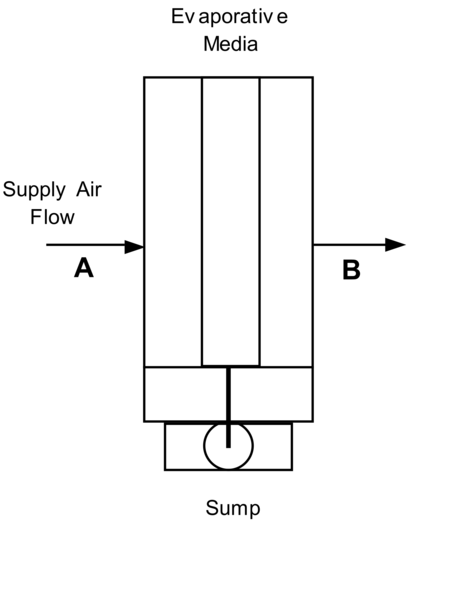
\includegraphics[width=0.9\textwidth, height=0.9\textheight, keepaspectratio=true]{media/image414.png}
\caption{Schematic of the ZoneHVAC:EnergyRecoveryVentilator compound object \protect \label{fig:schematic-of-the-zonehvac}}
\end{figure}

\subsubsection{Inputs}\label{inputs-3-006}

\paragraph{Field: Name}\label{field-name-3-006}

A unique user-assigned name for the stand alone ERV controller. Any reference to this controller by another object will use this name.

\paragraph{Field: Temperature High Limit}\label{field-temperature-high-limit}

The input for this field is the outdoor air temperature high limit ( °C) for economizer operation. If the outdoor air temperature is above this limit, economizer (free cooling) operation is terminated. No input (blank) in this field means that there is no outdoor air temperature high limit control.

\paragraph{Field: Temperature Low Limit}\label{field-temperature-low-limit}

The input for this field is the outdoor air temperature low limit ( °C) for economizer operation. If the outdoor air temperature is below this limit, economizer (free cooling) operation is terminated. No input (blank) in this field means that there is no outdoor air temperature low limit control.

\paragraph{Field: Enthalpy High Limit}\label{field-enthalpy-high-limit}

The input for this field is the outdoor air enthalpy limit (in J/kg) for economizer operation. If the outdoor air enthalpy is above this value, economizer (free cooling) operation is terminated. No input (blank) in this field means that there is no outdoor air economizer limit control.

\paragraph{Field: Dewpoint Temperature Limit}\label{field-dewpoint-temperature-limit}

Input for this field is the outdoor air dewpoint limit ( °C) for economizer operation. If the outdoor air dewpoint temperature is above this value, the outdoor airflow rate will be set to the minimum. No input (blank) in this field means that there is no outdoor air dewpoint limit control. This limit applies to the conditions at the Actuated Node regardless of whether or not there are any other components on the outdoor air path upstream of the mixer.

\paragraph{Field: Electronic Enthalpy Limit Curve Name}\label{field-electronic-enthalpy-limit-curve-name-1}

Input for this field is the name of a quadratic or cubic curve which provides the maximum outdoor air humidity ratio (function of outdoor air dry-bulb temperature) for economizer operation. If the outdoor air humidity ratio is greater than the curve's maximum humidity ratio (evaluated at the outdoor air dry-bulb temperature), the outdoor air flow rate will be set to the minimum. This limit applies to the conditions at the Actuated Node regardless of whether or not there are any other components on the outdoor air path upstream of the mixer. No input (blank) in this field means that there is no electronic enthalpy limit control.

\paragraph{Field: Exhaust Air Temperature Limit}\label{field-exhaust-air-temperature-limit}

This input establishes whether or not there is a limit control on the exhaust air temperature. The choices are \textbf{ExhaustAirTemperatureLimit} or \textbf{NoExhaustAirTemperatureLimit}. If \textbf{ExhaustAirTemperatureLimit} is chosen, the controller deactivates economizer mode whenever the outdoor air temperature is greater than the exhaust air temperature. If \textbf{NoExhaustAirTemperatureLimit} is chosen, no limit check on the exhaust air temperature is performed.

\paragraph{Field: Exhaust Air Enthalpy Limit}\label{field-exhaust-air-enthalpy-limit}

This input establishes whether or not there is a limit control on the exhaust air enthalpy. The choices are \textbf{ExhaustAirEnthalpyLimit} or \textbf{NoExhaustAirEnthalpyLimit}. If \textbf{ExhaustAirEnthalpyLimit} is chosen, the controller deactivates economizer mode whenever the outdoor air enthalpy is greater than the exhaust air enthalpy. If \textbf{NoExhaustAirEnthalpyLimit} is chosen, no limit check on the exhaust air enthalpy is performed.

\paragraph{Field: Time of Day Economizer Flow Control Schedule Name}\label{field-time-of-day-economizer-flow-control-schedule-name}

This alpha field is the name of a schedule which controls the change in air flow rate based on time-of-day. Schedule values equal to 0 disable this feature. Schedule values greater than 0 activate the economizer. Note that heat exchange between the air streams is suspended when the economizer is active. This schedule can be used with or without the high humidity control option. When an economizer is used in conjunction with the high humidity control option, high humidity control has priority.

\paragraph{Field: High Humidity Control Flag}\label{field-high-humidity-control-flag}

This optional choice field establishes whether or not the supply and exhaust air flow rates are modified in response to high indoor relative humidity. Valid choices are Yes and No. If Yes is selected, the supply and exhaust air flow rates may be modified when the indoor relative humidity is above the humidistat set point. If No is selected, this option is disabled and the following three fields are not used. Note that heat exchange between the air streams is suspended during times when high humidity control is active. The default value is No.

\paragraph{Field: Humidistat Control Zone Name}\label{field-humidistat-control-zone-name-1}

This optional input defines the zone name where the humidistat is located. This is the same zone name used in the Zone Control:Humidistat object. This field is required when the High Humidity Control Flag is specified as Yes.

\paragraph{Field: High Humidity Outdoor Air Flow Ratio}\label{field-high-humidity-outdoor-air-flow-ratio-1}

This optional input is the ratio of the modified supply (outdoor) air flow rate to the supply air flow rate specified in the Energy Recovery Ventilator:Stand Alone ERV object. When the high humidity control algorithm determines that the supply air flow rate will be changed (i.e.~increased or decreased), the operating supply air flow rate is equal to the supply air flow rate specified in the Energy Recovery Ventilator:Stand Alone ERV object multiplied by this ratio. The minimum value for this field is 0. This field is used to modify both the supply and exhaust air flow rates when high humidity control is active. The supply and exhaust air fan volumetric flow rates must be able to account for the increase in air flow when this input is greater than 1. The default value is 1.

\paragraph{Field: Control High Indoor Humidity based on Outdoor Humidity Ratio}\label{field-control-high-indoor-humidity-based-on-outdoor-humidity-ratio-1}

This optional choice field determines if high humidity control is activated based on high indoor relative humidity alone or is activated only when the indoor relative humidity is above the humidistat set point \emph{and} the outdoor humidity ratio is less than the indoor humidity ratio. Valid choices are Yes and No. If No is selected, high humidity control is active any time the zone humidistat senses a moisture load. If yes is selected, the model also verifies that the outdoor humidity ratio is less than the humidistat's zone air humidity ratio. This field is used only when the High Humidity Control Flag is specified as Yes. The default value is Yes.

Following is an example input for this stand alone ERV controller object:

\begin{lstlisting}

ZoneHVAC:EnergyRecoveryVentilator:Controller,
  ERV OA Controller 1,                       !- ERV controller name
  19.,                                                       !- Temperature high limit {C}
  14.,                                                       !- Temperature low limit {C}
  ,                                                             !- Enthalpy high limit {J/kg}
  15.55,                                                   !- dew point temperature limit (C)
  ElectronicEnthalpyCurveA,             !- electronic enthalpy limit curve name
  NoExhaustAirTemperatureLimit,     !- Exhaust air temperature limit
  NoExhaustAirEnthalpyLimit,           !- Exhaust air enthalpy limit
  OutsideAirFlowSchedule,                 !- Time of Day Economizer Flow Control Schedule Name
  Yes,                                                       !- High Humidity Control Flag
  East Zone,                                           !- Humidistat Control Zone Name
  1.2,                                                       !- High Humidity Outdoor air Flow Ratio
  Yes;                           !- Control High Indoor Humidity based on Outdoor Humidity Ratio


  Curve:Cubic,
  ElectronicEnthalpyCurveA, !- Name
  0.01342704,                             !- Coefficient1 Constant
  -0.00047892,                             !- Coefficient2 x
  0.000053352,                           !- Coefficient3 x**2
  -0.0000018103,                         !- Coefficient4 x**3
  16.6,                                         !- Minimum Value of x
  29.13;                                       !- Maximum Value of x
\end{lstlisting}
